\documentclass[slide]{../../custom}
\begin{document}

\begin{frame}
  \titlepage
\end{frame}

\begin{frame}
  \frametitle{摘要}
  \begin{itemize}
    \item \textbf{论文阅读与分析}
  \end{itemize}
\end{frame}

\begin{frame}
  \frametitle{论文阅读与分析}
  \cite{Wang2025} 文中详细阐述了针对HT树、FORS树及WOTS+算法的并行化策略,并依据各组成部分的执行顺序提出了一种分层并行方案,共划分为四个层次。由于各层之间相对独立,该文提出的组合并行策略可根据具体资源情况灵活调整,从而实现\textcolor{blue}{更高的并行效率(PE)},即 PE=效率/资源。

\end{frame}

\begin{frame}
  \frametitle{Merkle Tree 并行化}
  如图 \ref{fig:merkle_tree_paralle} 所示,左侧示例展示了最大并行化情形,即将每次HASH运算视为独立任务,但由此引入了四次同步操作,导致计算负载不均衡并引发等待现象;而右侧示例则采用最小并行化策略,将所有HASH运算合并为两个任务,虽然有效缓解了负载不均问题,但并行度则显著降低。因此,我们计划在这两种策略之间寻求一个\textcolor{blue}{合适的HASH运算分组数},以实现计算负载与并行度之间的最佳折中,并由此提升PE。
  \begin{figure}[!ht]
    \centering
    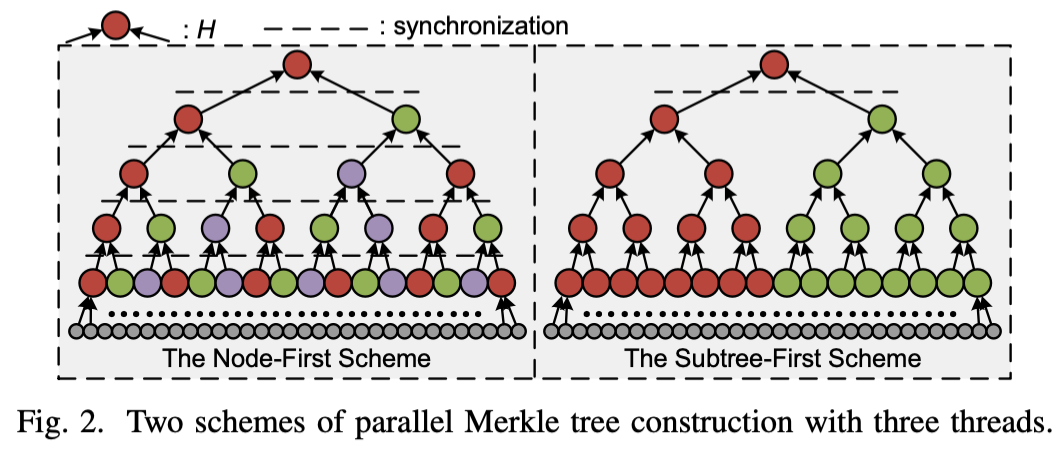
\includegraphics[width=0.6\textwidth]{./fig/merkle_tree_paralle.png}
    \caption{Merkle Tree 并行化\cite{Wang2025}}
    \label{fig:merkle_tree_paralle}
  \end{figure}
\end{frame}

\begin{frame}
  \frametitle{老师评语}
  \begin{alertblock}{阴影标注部分需要更详细说明创新,而不是如此简单,现在的摘要是没有意义的}
    现确定创新的方向为:更高的并行效率(PE)和签名算法的场景应用,创新手段确定后,再对摘要进行修改。
  \end{alertblock}
  \begin{alertblock}{论文写作基本没有推进 ??}
    在精读\cite{Wang2025}论文与代码花费太多时间。
  \end{alertblock}

  \begin{block}{下周计划}
    \begin{itemize}
      \item 复现 \cite{Wang2025} 实验
      \item 调整HASH运算分组数,提升并行效率 PE
    \end{itemize}
  \end{block}
\end{frame}

\begin{frame}
  \frametitle{参考文献}
  \bibliographystyle{alpha}
  \bibliography{../../paper}
\end{frame}

\end{document}